% Options for packages loaded elsewhere
\PassOptionsToPackage{unicode}{hyperref}
\PassOptionsToPackage{hyphens}{url}
\documentclass[
]{article}
\usepackage{xcolor}
\usepackage{amsmath,amssymb}
\setcounter{secnumdepth}{-\maxdimen} % remove section numbering
\usepackage{iftex}
\ifPDFTeX
  \usepackage[T1]{fontenc}
  \usepackage[utf8]{inputenc}
  \usepackage{textcomp} % provide euro and other symbols
\else % if luatex or xetex
  \usepackage{unicode-math} % this also loads fontspec
  \defaultfontfeatures{Scale=MatchLowercase}
  \defaultfontfeatures[\rmfamily]{Ligatures=TeX,Scale=1}
\fi
\usepackage{lmodern}
\ifPDFTeX\else
  % xetex/luatex font selection
\fi
% Use upquote if available, for straight quotes in verbatim environments
\IfFileExists{upquote.sty}{\usepackage{upquote}}{}
\IfFileExists{microtype.sty}{% use microtype if available
  \usepackage[]{microtype}
  \UseMicrotypeSet[protrusion]{basicmath} % disable protrusion for tt fonts
}{}
\makeatletter
\@ifundefined{KOMAClassName}{% if non-KOMA class
  \IfFileExists{parskip.sty}{%
    \usepackage{parskip}
  }{% else
    \setlength{\parindent}{0pt}
    \setlength{\parskip}{6pt plus 2pt minus 1pt}}
}{% if KOMA class
  \KOMAoptions{parskip=half}}
\makeatother
\usepackage{color}
\usepackage{fancyvrb}
\newcommand{\VerbBar}{|}
\newcommand{\VERB}{\Verb[commandchars=\\\{\}]}
\DefineVerbatimEnvironment{Highlighting}{Verbatim}{commandchars=\\\{\}}
% Add ',fontsize=\small' for more characters per line
\newenvironment{Shaded}{}{}
\newcommand{\AlertTok}[1]{\textcolor[rgb]{1.00,0.00,0.00}{\textbf{#1}}}
\newcommand{\AnnotationTok}[1]{\textcolor[rgb]{0.38,0.63,0.69}{\textbf{\textit{#1}}}}
\newcommand{\AttributeTok}[1]{\textcolor[rgb]{0.49,0.56,0.16}{#1}}
\newcommand{\BaseNTok}[1]{\textcolor[rgb]{0.25,0.63,0.44}{#1}}
\newcommand{\BuiltInTok}[1]{\textcolor[rgb]{0.00,0.50,0.00}{#1}}
\newcommand{\CharTok}[1]{\textcolor[rgb]{0.25,0.44,0.63}{#1}}
\newcommand{\CommentTok}[1]{\textcolor[rgb]{0.38,0.63,0.69}{\textit{#1}}}
\newcommand{\CommentVarTok}[1]{\textcolor[rgb]{0.38,0.63,0.69}{\textbf{\textit{#1}}}}
\newcommand{\ConstantTok}[1]{\textcolor[rgb]{0.53,0.00,0.00}{#1}}
\newcommand{\ControlFlowTok}[1]{\textcolor[rgb]{0.00,0.44,0.13}{\textbf{#1}}}
\newcommand{\DataTypeTok}[1]{\textcolor[rgb]{0.56,0.13,0.00}{#1}}
\newcommand{\DecValTok}[1]{\textcolor[rgb]{0.25,0.63,0.44}{#1}}
\newcommand{\DocumentationTok}[1]{\textcolor[rgb]{0.73,0.13,0.13}{\textit{#1}}}
\newcommand{\ErrorTok}[1]{\textcolor[rgb]{1.00,0.00,0.00}{\textbf{#1}}}
\newcommand{\ExtensionTok}[1]{#1}
\newcommand{\FloatTok}[1]{\textcolor[rgb]{0.25,0.63,0.44}{#1}}
\newcommand{\FunctionTok}[1]{\textcolor[rgb]{0.02,0.16,0.49}{#1}}
\newcommand{\ImportTok}[1]{\textcolor[rgb]{0.00,0.50,0.00}{\textbf{#1}}}
\newcommand{\InformationTok}[1]{\textcolor[rgb]{0.38,0.63,0.69}{\textbf{\textit{#1}}}}
\newcommand{\KeywordTok}[1]{\textcolor[rgb]{0.00,0.44,0.13}{\textbf{#1}}}
\newcommand{\NormalTok}[1]{#1}
\newcommand{\OperatorTok}[1]{\textcolor[rgb]{0.40,0.40,0.40}{#1}}
\newcommand{\OtherTok}[1]{\textcolor[rgb]{0.00,0.44,0.13}{#1}}
\newcommand{\PreprocessorTok}[1]{\textcolor[rgb]{0.74,0.48,0.00}{#1}}
\newcommand{\RegionMarkerTok}[1]{#1}
\newcommand{\SpecialCharTok}[1]{\textcolor[rgb]{0.25,0.44,0.63}{#1}}
\newcommand{\SpecialStringTok}[1]{\textcolor[rgb]{0.73,0.40,0.53}{#1}}
\newcommand{\StringTok}[1]{\textcolor[rgb]{0.25,0.44,0.63}{#1}}
\newcommand{\VariableTok}[1]{\textcolor[rgb]{0.10,0.09,0.49}{#1}}
\newcommand{\VerbatimStringTok}[1]{\textcolor[rgb]{0.25,0.44,0.63}{#1}}
\newcommand{\WarningTok}[1]{\textcolor[rgb]{0.38,0.63,0.69}{\textbf{\textit{#1}}}}
\usepackage{graphicx}
\makeatletter
\newsavebox\pandoc@box
\newcommand*\pandocbounded[1]{% scales image to fit in text height/width
  \sbox\pandoc@box{#1}%
  \Gscale@div\@tempa{\textheight}{\dimexpr\ht\pandoc@box+\dp\pandoc@box\relax}%
  \Gscale@div\@tempb{\linewidth}{\wd\pandoc@box}%
  \ifdim\@tempb\p@<\@tempa\p@\let\@tempa\@tempb\fi% select the smaller of both
  \ifdim\@tempa\p@<\p@\scalebox{\@tempa}{\usebox\pandoc@box}%
  \else\usebox{\pandoc@box}%
  \fi%
}
% Set default figure placement to htbp
\def\fps@figure{htbp}
\makeatother
\setlength{\emergencystretch}{3em} % prevent overfull lines
\providecommand{\tightlist}{%
  \setlength{\itemsep}{0pt}\setlength{\parskip}{0pt}}
\usepackage{bookmark}
\IfFileExists{xurl.sty}{\usepackage{xurl}}{} % add URL line breaks if available
\urlstyle{same}
\hypersetup{
  hidelinks,
  pdfcreator={LaTeX via pandoc}}

\author{}
\date{}

\begin{document}

\section{WebGAL Transform Editor}\label{webgal-transform-editor}

🎥 基于 \href{https://tauri.app}{Tauri} +
\href{https://react.dev}{React} +
\href{https://www.typescriptlang.org/}{TypeScript} 开发的 WebGAL
运镜脚本编辑器。\\
支持可视化设置立绘位置、缩放、旋转(弧度),并导出 \texttt{setTransform}
与 \texttt{changeFigure} 指令!

\begin{center}\rule{0.5\linewidth}{0.5pt}\end{center}

\subsection{✨ 功能特色}\label{ux529fux80fdux7279ux8272}

\subsubsection{🎯
核心编辑功能}\label{ux6838ux5fc3ux7f16ux8f91ux529fux80fd}

\begin{itemize}
\tightlist
\item
  ✅ 支持解析与编辑 \texttt{setTransform} 脚本(位置、缩放、旋转)
\item
  ✅ 支持 \texttt{changeFigure} 指令编辑与导出(motion / expression / id
  / transform)
\item
  ✅ 增量合并:\texttt{setTransform} 命令支持继承上一句的属性值
\item
  ✅ 实时导出 WebGAL 脚本片段
\end{itemize}

\subsubsection{🖱️ 交互操作}\label{ux4ea4ux4e92ux64cdux4f5c}

\begin{itemize}
\tightlist
\item
  ✅ \textbf{鼠标拖拽}:自由移动模型位置
\item
  ✅ \textbf{缩放}:\texttt{Ctrl\ +\ 鼠标滚轮} 缩放模型
\item
  ✅ \textbf{旋转}:\texttt{Alt\ +\ 鼠标拖拽} 旋转模型,体验类似
  Photoshop 旋转控件
\item
  ✅ \textbf{多选}:\texttt{Shift\ +\ 点击} 选中多个模型
\item
  ✅ \textbf{全选/取消全选}:使用工具栏按钮快速选择所有模型
\end{itemize}

\subsubsection{🎮 WebGAL 模式}\label{webgal-ux6a21ux5f0f}

\begin{itemize}
\tightlist
\item
  ✅ 连接 WebGAL 游戏文件夹,自动识别 \texttt{figure} 和
  \texttt{background} 目录
\item
  ✅ 可视化选择立绘和背景文件
\item
  ✅ 一键加载游戏资源,无需手动复制文件路径
\item
  ✅ 支持 Live2D 模型(\texttt{.json} 和 \texttt{.jsonl} 格式)
\end{itemize}

\subsubsection{👁️ 观测层功能}\label{ux89c2ux6d4bux5c42ux529fux80fd}

\begin{itemize}
\tightlist
\item
  ✅
  \textbf{颜色层}:在场景上覆盖一层中性灰,混合模式为颜色,用于观测明度。
\item
  ✅
  \textbf{明度层}:在场景上覆盖一层中性灰,混合模式为明度,用于观测颜色。
\item
  ⚠️
  \textbf{注意}:开启观测层时,画布会阻止交互,无法拖拽或旋转模型(用于纯粹查看效果)
\end{itemize}

\subsubsection{📏 辅助线功能}\label{ux8f85ux52a9ux7ebfux529fux80fd}

\begin{itemize}
\tightlist
\item
  ✅ \textbf{无辅助线}:关闭辅助线显示
\item
  ✅ \textbf{三分法}:显示三分法构图辅助线
\item
  ✅ \textbf{中心十字}:显示中心十字辅助线
\item
  ✅ \textbf{对角线}:显示对角线辅助线
\item
  ✅ \textbf{黄金比例}:显示黄金比例辅助线
\end{itemize}

\subsubsection{🎨 滤镜系统}\label{ux6ee4ux955cux7cfbux7edf}

\begin{itemize}
\tightlist
\item
  ✅ 丰富的内置滤镜预设(模糊、老电影、噪点、反射、RGB分离等)
\item
  ✅ 自定义滤镜参数调整
\item
  ✅ 支持保存和加载用户预设
\item
  ✅ 可选择应用到所有模型或仅选中模型
\end{itemize}

\begin{center}\rule{0.5\linewidth}{0.5pt}\end{center}

\subsection{🚀 快速开始}\label{ux5febux901fux5f00ux59cb}

\subsubsection{1. 克隆项目}\label{ux514bux9686ux9879ux76ee}

\begin{Shaded}
\begin{Highlighting}[]
\FunctionTok{git}\NormalTok{ clone https://github.com/KonshinHaoshin/Webgal\_transformEditor.git}
\BuiltInTok{cd}\NormalTok{ Webgal\_transformEditor}
\end{Highlighting}
\end{Shaded}

\subsubsection{2. 安装依赖}\label{ux5b89ux88c5ux4f9dux8d56}

本项目使用 npm 作为包管理器

\begin{Shaded}
\begin{Highlighting}[]
\ExtensionTok{npm}\NormalTok{ install}
\end{Highlighting}
\end{Shaded}

\subsubsection{3.
启动开发环境}\label{ux542fux52a8ux5f00ux53d1ux73afux5883}

\begin{Shaded}
\begin{Highlighting}[]
\ExtensionTok{npm}\NormalTok{ run tauri dev}
\end{Highlighting}
\end{Shaded}

启动后自动打开桌面窗口,进行可视化脚本编辑。

\begin{center}\rule{0.5\linewidth}{0.5pt}\end{center}

\subsection{📖 详细使用方法}\label{ux8be6ux7ec6ux4f7fux7528ux65b9ux6cd5}

\subsubsection{🖱️ 基础操作}\label{ux57faux7840ux64cdux4f5c}

\paragraph{移动模型}\label{ux79fbux52a8ux6a21ux578b}

\begin{enumerate}
\def\labelenumi{\arabic{enumi}.}
\tightlist
\item
  \textbf{单选移动}:直接点击并拖拽模型
\item
  \textbf{多选移动}:

  \begin{itemize}
  \tightlist
  \item
    按住 \texttt{Shift} 键,依次点击需要选中的模型
  \item
    或者点击 “Select All” 按钮全选所有模型
  \item
    选中后拖拽任意一个模型,所有选中的模型会同步移动
  \end{itemize}
\end{enumerate}

\paragraph{缩放模型}\label{ux7f29ux653eux6a21ux578b}

\begin{itemize}
\tightlist
\item
  按住 \texttt{Ctrl} 键,然后滚动鼠标滚轮
\item
  \textbf{向上滚动}:放大模型
\item
  \textbf{向下滚动}:缩小模型
\item
  缩放会相对于鼠标位置进行,提供更精确的缩放体验
\end{itemize}

\paragraph{旋转模型}\label{ux65cbux8f6cux6a21ux578b}

\begin{itemize}
\tightlist
\item
  按住 \texttt{Alt} 键,然后拖拽模型
\item
  旋转会围绕模型中心点进行
\item
  旋转角度以弧度为单位显示(后续会转换为度数的显示)
\end{itemize}

\paragraph{选择操作}\label{ux9009ux62e9ux64cdux4f5c}

\begin{itemize}
\tightlist
\item
  \textbf{单选}:直接点击模型
\item
  \textbf{多选}:按住 \texttt{Shift} 键,点击多个模型
\item
  \textbf{全选}:点击工具栏的 “Select All” 按钮
\item
  \textbf{取消全选}:点击工具栏的 “Deselect All” 按钮
\end{itemize}

\subsubsection{🎮 WebGAL
模式使用}\label{webgal-ux6a21ux5f0fux4f7fux7528}

\begin{enumerate}
\def\labelenumi{\arabic{enumi}.}
\tightlist
\item
  \textbf{启用 WebGAL 模式}:

  \begin{itemize}
  \tightlist
  \item
    勾选界面上的 “WebGAL模式” 复选框
  \item
    在弹出的文件夹选择对话框中选择你的 WebGAL 游戏根目录
  \end{itemize}
\item
  \textbf{加载资源}:

  \begin{itemize}
  \tightlist
  \item
    在 WebGAL 模式下,可以方便地选择 \texttt{figure} 目录中的立绘文件
  \item
    支持普通图片格式(\texttt{.png}、\texttt{.jpg} 等)和 Live2D
    模型(\texttt{.json}、\texttt{.jsonl})
  \item
    选择背景文件时,会从 \texttt{background} 目录中加载
  \end{itemize}
\item
  \textbf{Live2D 支持}:

  \begin{itemize}
  \tightlist
  \item
    支持且只支持cubism2类型的live2d文件(常见的如你邦的live2d)
  \item
    支持社区中存在的compositeModel模型(jsonl聚合模型)
  \item
    加载后可以在画布上预览和编辑 Live2D 模型的变换
  \item
    支持 Live2D 模型的移动、缩放和旋转操作
  \item
    目前暂未实现显示live2d动作标签
  \end{itemize}
\item
  \textbf{退出 WebGAL 模式}:

  \begin{itemize}
  \tightlist
  \item
    取消勾选 “WebGAL模式” 复选框即可退出
    \pandocbounded{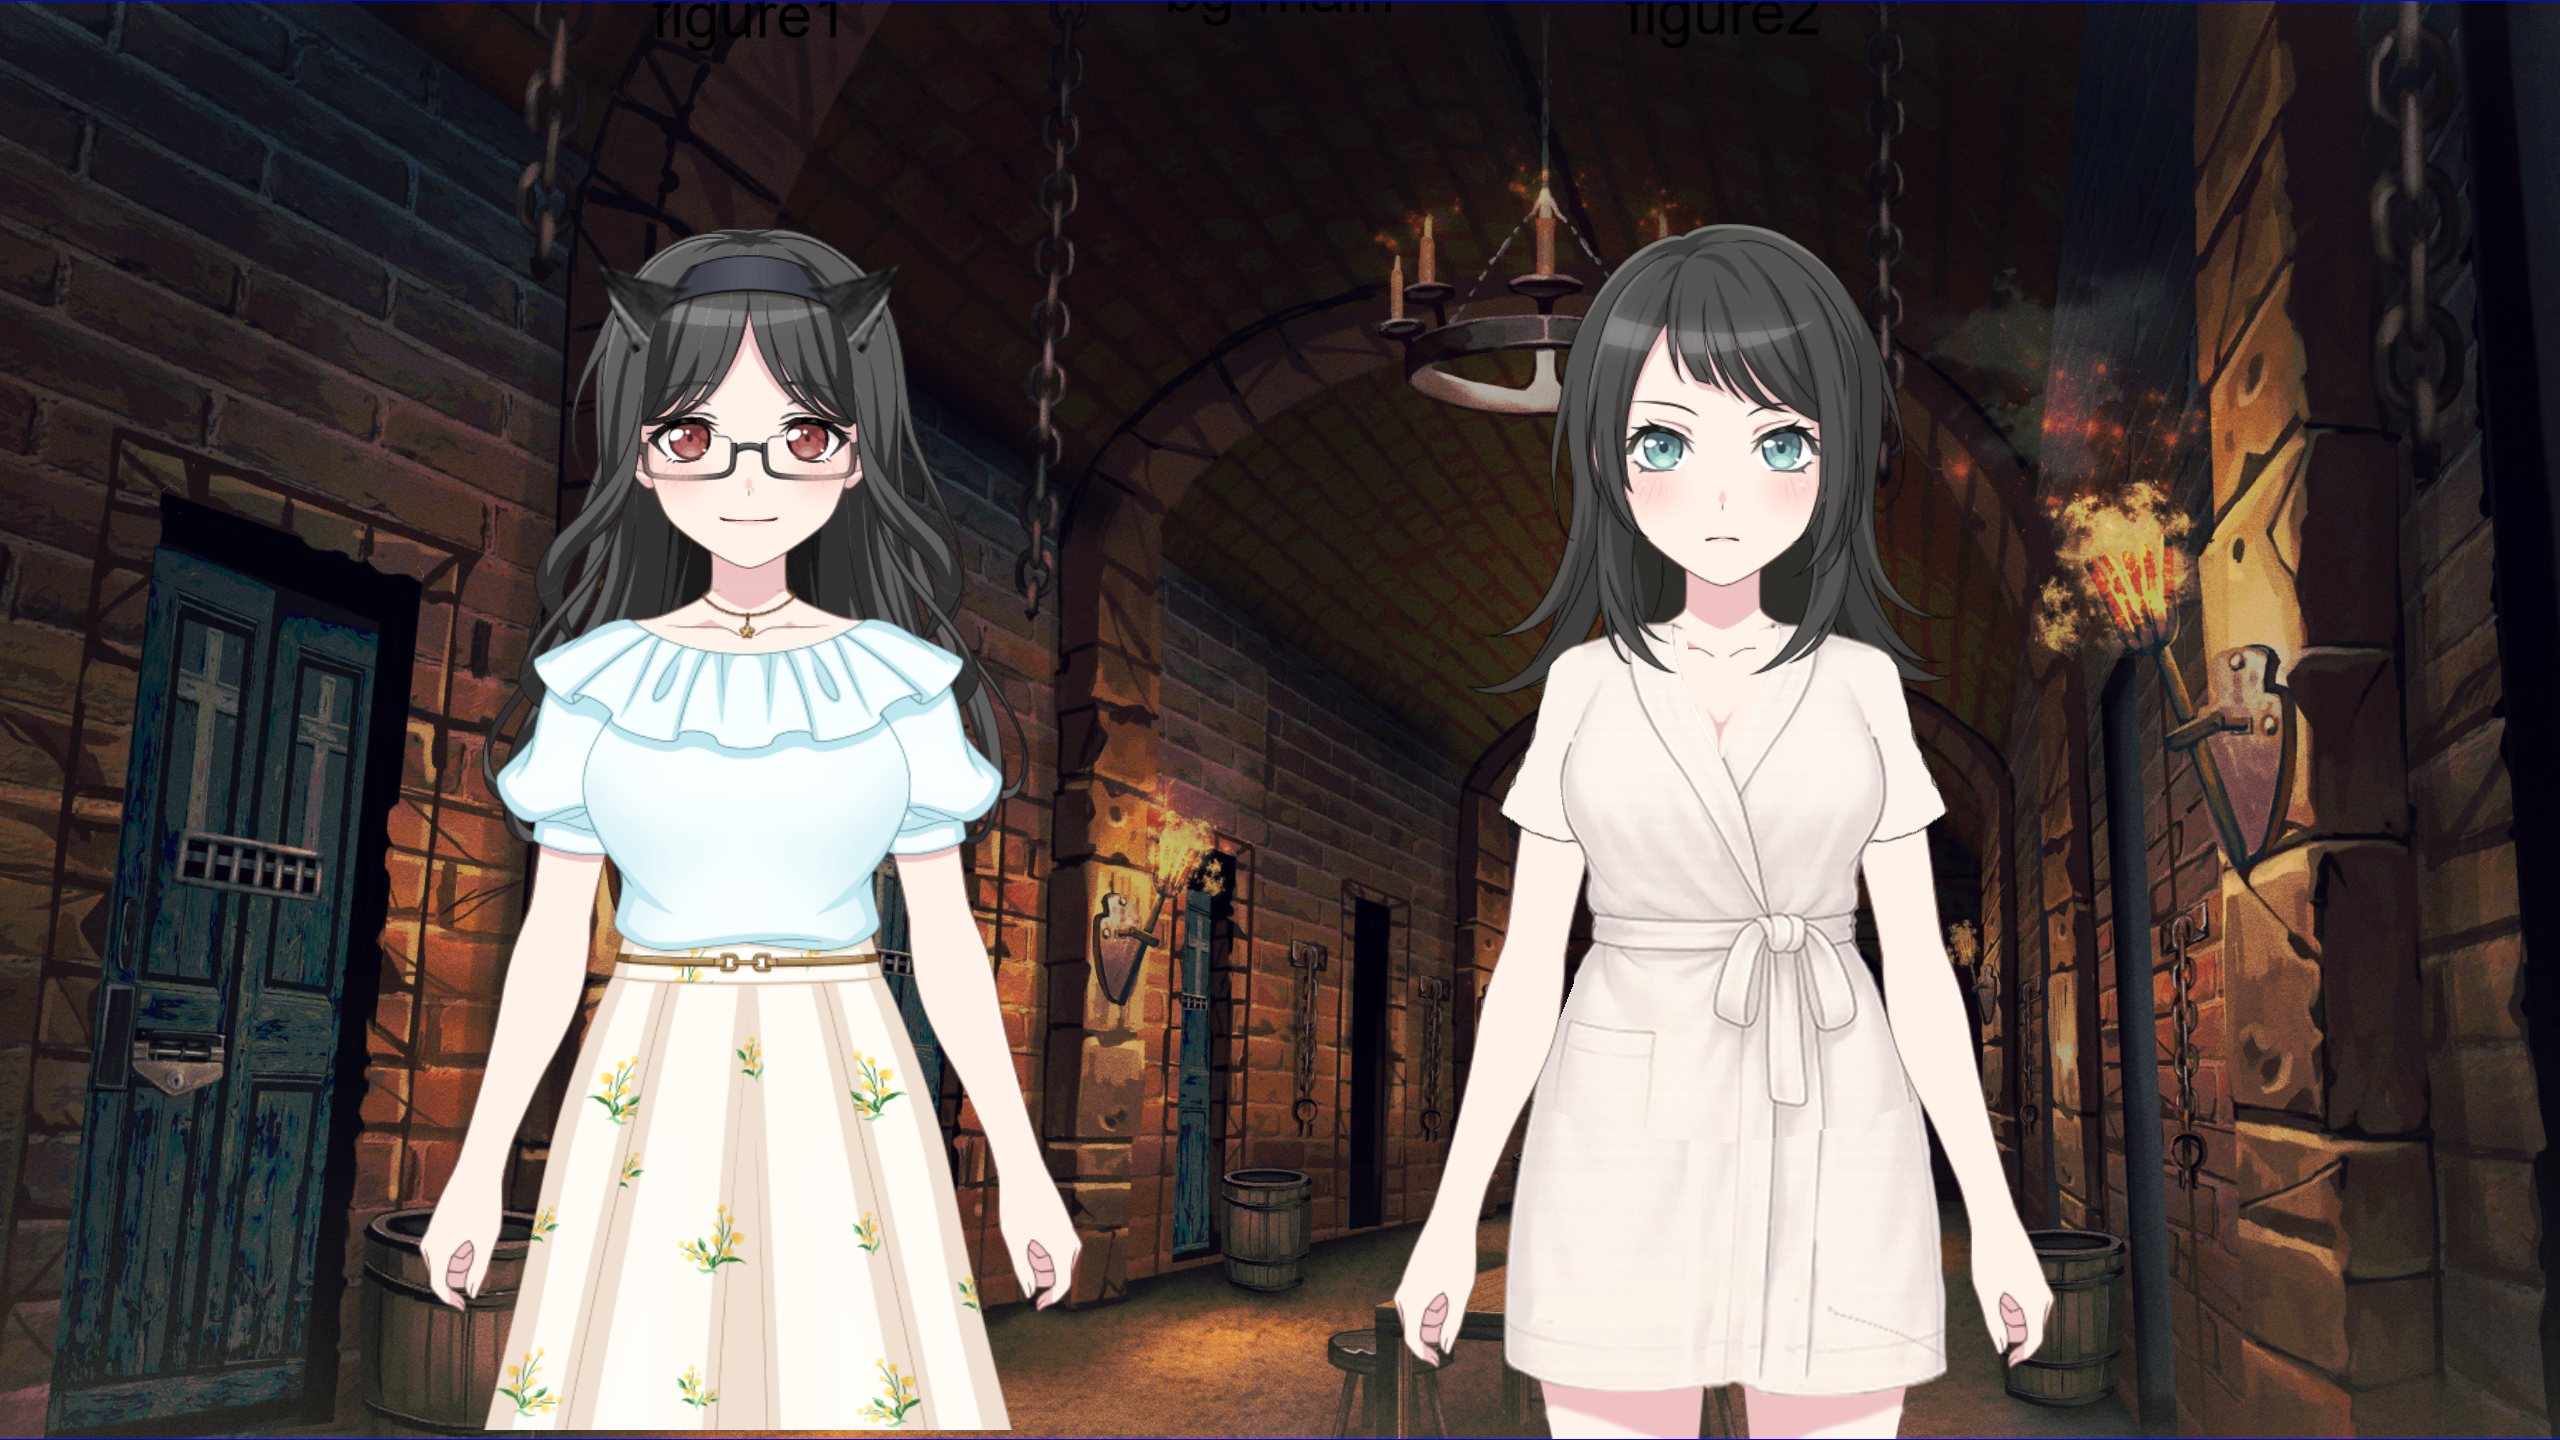
\includegraphics[keepaspectratio,alt={Webgal模式示意图}]{./media-223389ac98cc9354/readme/test1.png}}
    \textgreater{}
    webgal模式示意图如上,其中左边的是由b站up主哈吉拉克上的岸古制作的号角soyo.jsonl,旁边的浴袍则是群u制作的浴袍海玲.json
  \end{itemize}
\end{enumerate}

\subsubsection{👁️
观测层功能使用}\label{ux89c2ux6d4bux5c42ux529fux80fdux4f7fux7528}

\begin{enumerate}
\def\labelenumi{\arabic{enumi}.}
\tightlist
\item
  \textbf{开启观测层}:

  \begin{itemize}
  \tightlist
  \item
    在顶部工具栏找到 “观察层” 下拉菜单
  \item
    选择 “颜色” 或 “明度” 模式
  \end{itemize}
\item
  \textbf{查看效果}:

  \begin{itemize}
  \tightlist
  \item
    场景会实时转换为对应的观测模式显示
  \item
    便于检查构图的色彩分布或明度层次
  \end{itemize}
\item
  \textbf{注意事项}:

  \begin{itemize}
  \tightlist
  \item
    ⚠️ \textbf{开启观测层时,画布会阻止所有交互}(包括拖拽、旋转、缩放)
  \item
    这是设计特性,目的是让你专注于查看效果而不误操作
  \end{itemize}
\item
  \textbf{关闭观测层}:

  \begin{itemize}
  \tightlist
  \item
    在 “观察层” 下拉菜单中选择 “无” 即可恢复正常显示和交互
  \end{itemize}
\end{enumerate}

\pandocbounded{\includegraphics[keepaspectratio,alt={颜色模式示意图}]{./media-223389ac98cc9354/readme/test2.png}}
\pandocbounded{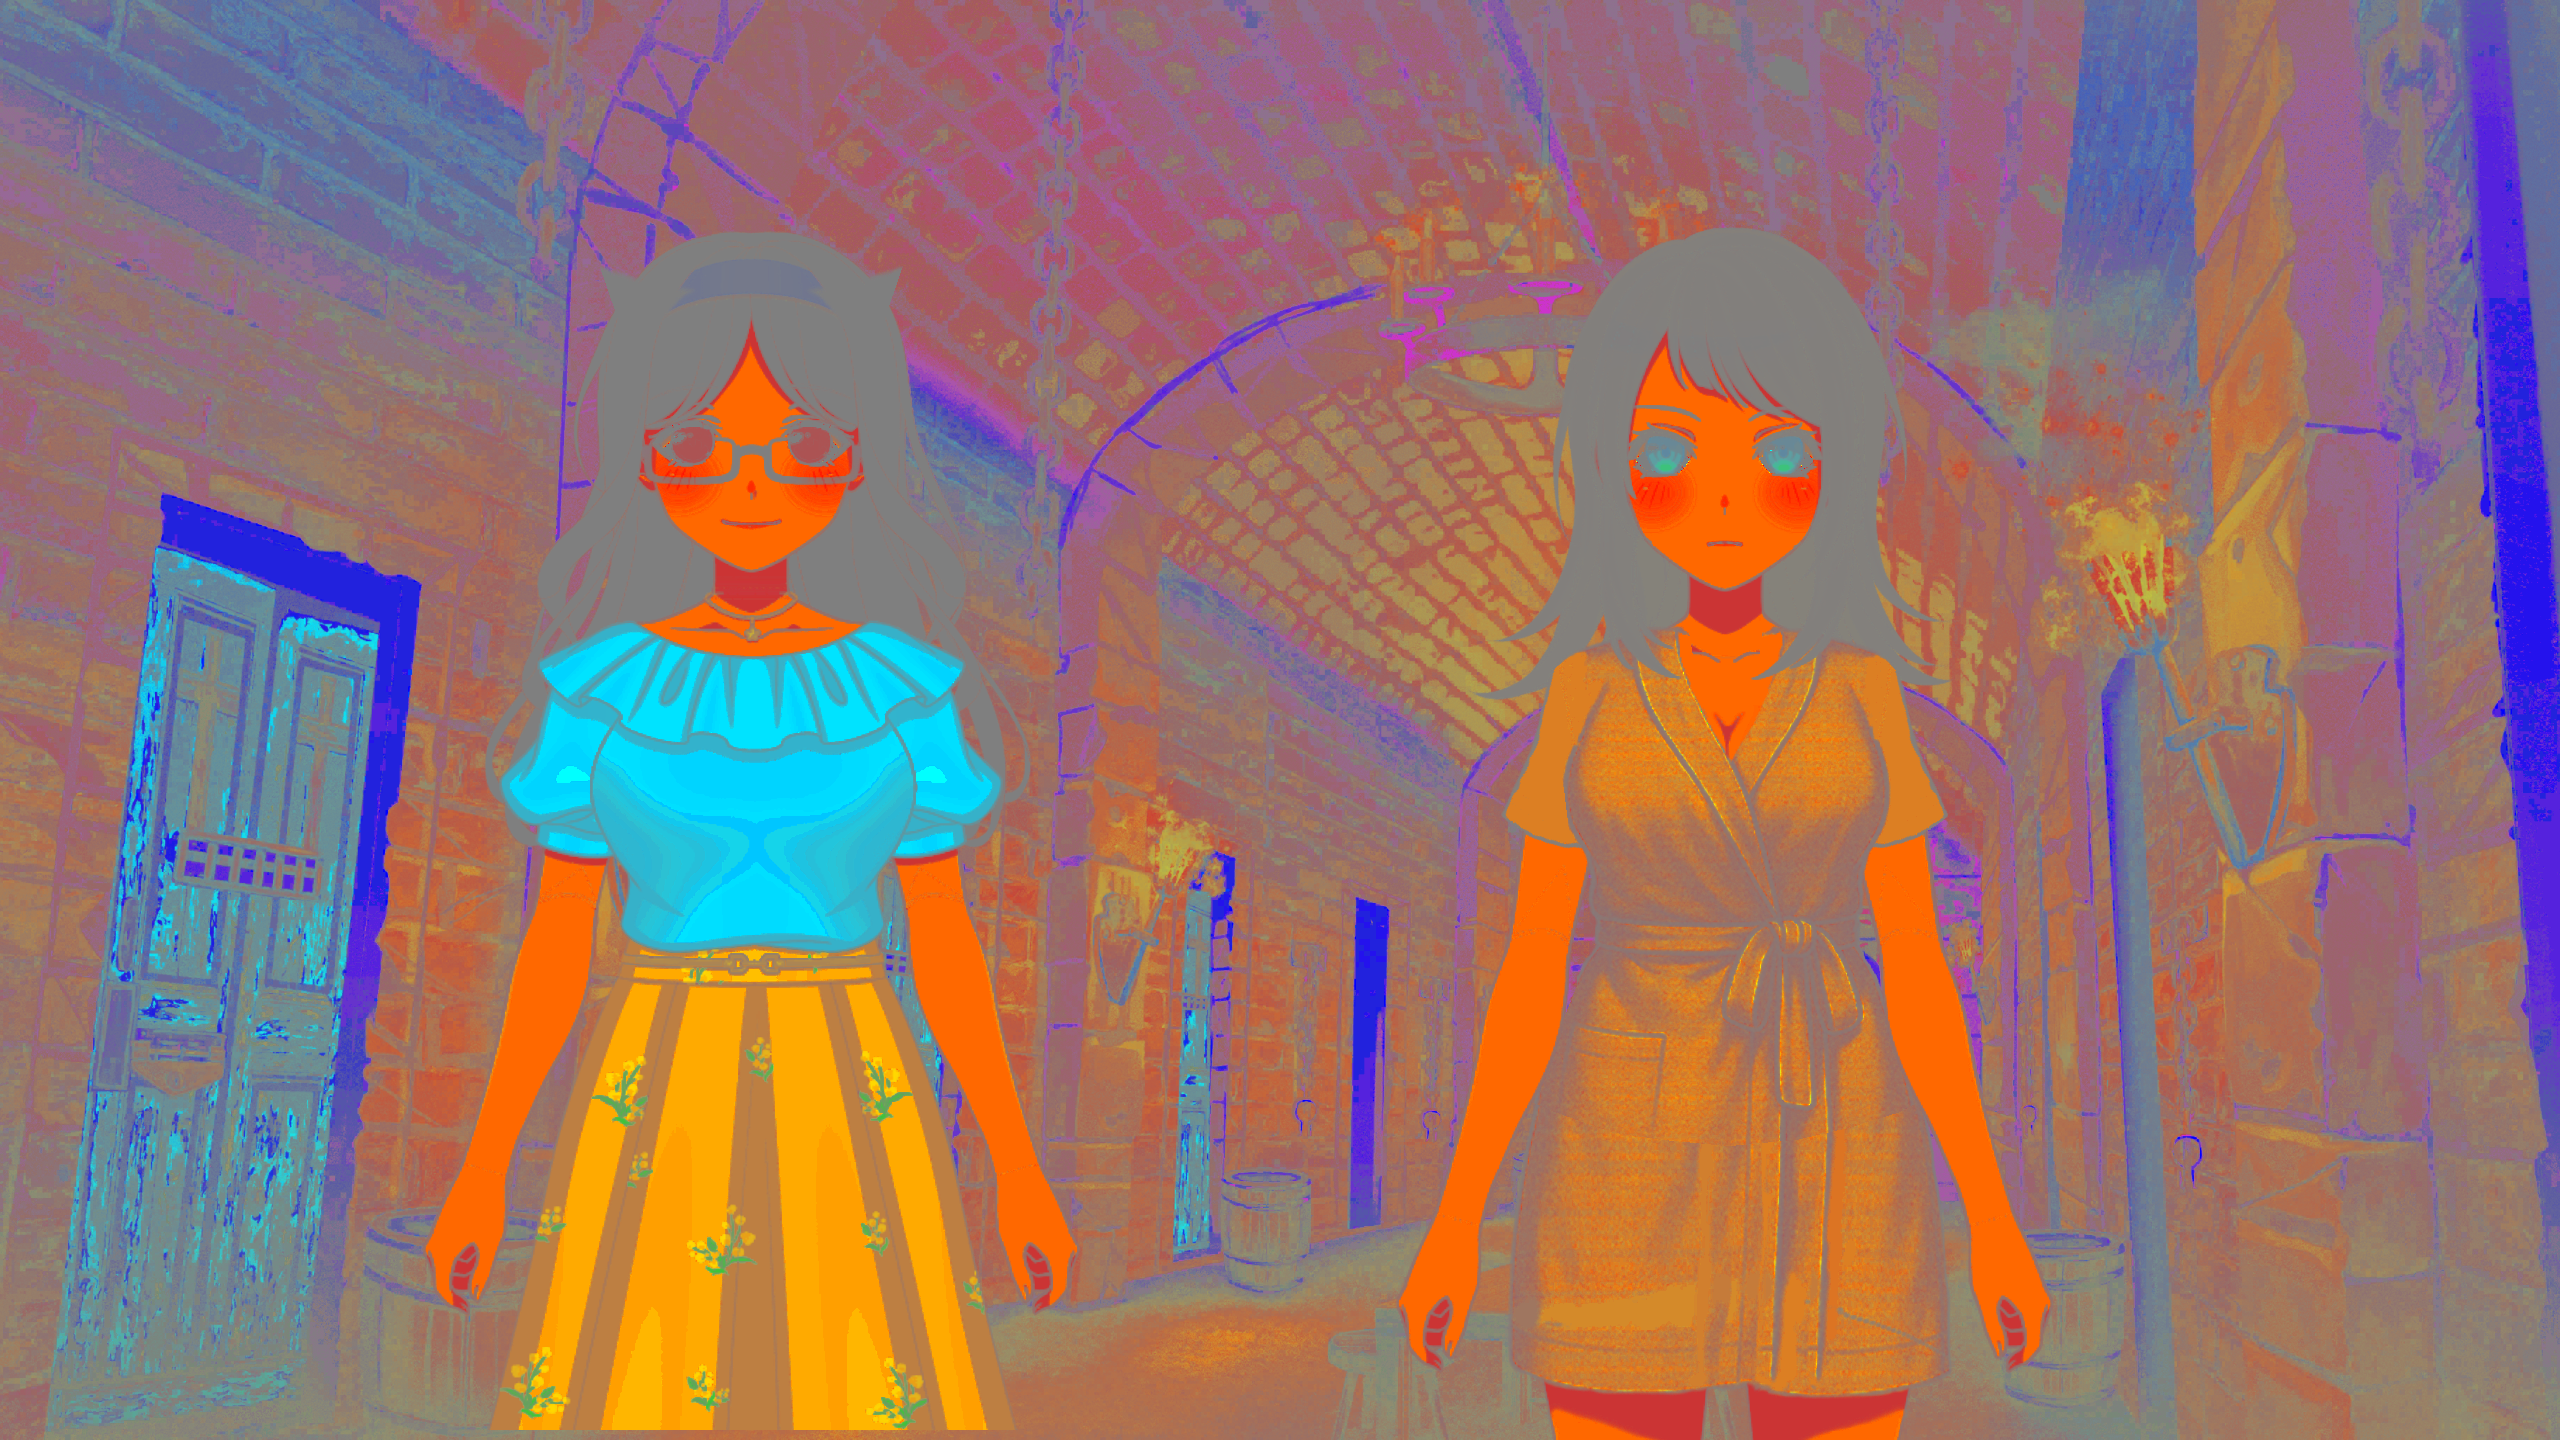
\includegraphics[keepaspectratio,alt={明度模式示意图}]{./media-223389ac98cc9354/readme/test3.png}}
\textgreater{} 第一个是颜色模式的示意图,第二个是明度模式的示意图……
\textgreater{}
是的,颜色模式是用来观察明度的,明度模式是用来观察颜色的。至于为什么我要这么命名,只是因为中性灰这一层的混合模式罢了……

\subsubsection{📏
辅助线功能使用}\label{ux8f85ux52a9ux7ebfux529fux80fdux4f7fux7528}

\begin{enumerate}
\def\labelenumi{\arabic{enumi}.}
\tightlist
\item
  \textbf{选择辅助线类型}:

  \begin{itemize}
  \tightlist
  \item
    在顶部工具栏找到 “辅助线” 下拉菜单
  \item
    选择需要的辅助线类型:

    \begin{itemize}
    \tightlist
    \item
      \textbf{无辅助线}:关闭辅助线
    \item
      \textbf{三分法}:显示三分法构图线,适合突出主体
    \item
      \textbf{中心十字}:显示中心十字线,适合对称构图
    \item
      \textbf{对角线}:显示对角线,适合动态构图
    \item
      \textbf{黄金比例}:显示黄金比例线,适合经典构图
    \end{itemize}
  \end{itemize}
\item
  \textbf{使用技巧}:

  \begin{itemize}
  \tightlist
  \item
    辅助线会叠加显示在画布上,不会影响实际操作
  \item
    可以随时切换不同的辅助线类型来比较效果
  \item
    建议在最终确定位置前使用辅助线检查构图
  \end{itemize}
\end{enumerate}

\subsubsection{🎨
滤镜功能使用}\label{ux6ee4ux955cux529fux80fdux4f7fux7528}

\begin{enumerate}
\def\labelenumi{\arabic{enumi}.}
\tightlist
\item
  \textbf{应用滤镜预设}:

  \begin{itemize}
  \tightlist
  \item
    勾选 “启用滤镜预设” 复选框
  \item
    在滤镜预设下拉菜单中选择预设
  \item
    点击 “应用到选中模型” 或 “应用到所有模型”
  \item
    后续可能会更新hsl模式
  \end{itemize}
\item
  \textbf{自定义滤镜}:

  \begin{itemize}
  \tightlist
  \item
    调整右侧滤镜面板中的各项参数
  \item
    参数会实时应用到画布上
  \end{itemize}
\item
  \textbf{保存自定义预设}:

  \begin{itemize}
  \tightlist
  \item
    调整好滤镜参数后,可以在滤镜面板中保存为自定义预设
  \item
    自定义预设会保存到浏览器本地存储中
  \end{itemize}
\item
  \textbf{应用范围}:

  \begin{itemize}
  \tightlist
  \item
    \textbf{应用到选中模型}:仅将滤镜应用到当前选中的模型
  \item
    \textbf{应用到所有模型}:将滤镜应用到画布上的所有模型(包括背景)
    \pandocbounded{\includegraphics[keepaspectratio,alt={滤镜编辑器示意图}]{./media-223389ac98cc9354/readme/test4.png}}
    \textgreater{} 效果如下
    \pandocbounded{\includegraphics[keepaspectratio,alt={预设示意图}]{./media-223389ac98cc9354/readme/test5.png}}
    \textgreater{} 为了方便大家使用,我制作了大量的滤镜预设
  \end{itemize}
\end{enumerate}

\subsubsection{📝 脚本编辑}\label{ux811aux672cux7f16ux8f91}

\begin{enumerate}
\def\labelenumi{\arabic{enumi}.}
\tightlist
\item
  \textbf{解析脚本}:

  \begin{itemize}
  \tightlist
  \item
    在左侧文本框中粘贴 WebGAL 脚本
  \item
    点击 “Load Script” 按钮,会自动打开输出脚本界面
  \item
    脚本会被解析并在画布上显示对应的模型和变换
  \end{itemize}
\item
  \textbf{编辑脚本}:

  \begin{itemize}
  \tightlist
  \item
    在输出脚本窗口中,可以直接编辑每一行脚本
  \item
    \textbf{实时同步}:编辑脚本后,主窗口会实时更新显示效果
  \item
    \textbf{添加/移除 \texttt{-next}}:点击每行左侧的 “N”
    按钮可以添加或移除 \texttt{-next} 标记
  \item
    \textbf{设置断点}:点击每行左侧的 “○”
    按钮可以设置断点,用于调试动画播放
  \item
    \textbf{删除行}:点击每行右侧的 “×” 按钮可以删除该行脚本
  \item
    \textbf{复制脚本}:

    \begin{itemize}
    \tightlist
    \item
      点击 “复制脚本” 按钮可以复制所有脚本
    \item
      点击 “只复制setTransform语句” 按钮可以只复制 \texttt{setTransform}
      命令
    \end{itemize}
  \item
    \textbf{快捷键}:

    \begin{itemize}
    \tightlist
    \item
      \texttt{Enter}:提交编辑并应用更改
    \item
      \texttt{Shift\ +\ Enter}:在脚本行中插入换行
    \end{itemize}
  \end{itemize}
\item
  \textbf{脚本导出}:

  \begin{itemize}
  \tightlist
  \item
    脚本会自动实时导出到输出脚本窗口
  \item
    支持导出 \texttt{setTransform} 和 \texttt{changeFigure} 指令
  \item
    可以设置导出动画的持续时间(duration)和缓动函数(ease)
  \item
    支持增量合并:\texttt{setTransform} 命令会继承上一句的属性值
  \end{itemize}
\end{enumerate}

\subsubsection{🎬 动画预览}\label{ux52a8ux753bux9884ux89c8}

\begin{enumerate}
\def\labelenumi{\arabic{enumi}.}
\tightlist
\item
  \textbf{播放动画}:

  \begin{itemize}
  \tightlist
  \item
    点击 “播放” 按钮可以预览脚本动画效果
  \item
    动画会按照脚本中的时间顺序播放
  \item
    播放过程中会显示动画的实时状态
  \end{itemize}
\item
  \textbf{断点调试}:

  \begin{itemize}
  \tightlist
  \item
    在输出脚本窗口中设置断点
  \item
    动画播放会在断点处暂停
  \item
    可以检查每个关键帧的效果
  \end{itemize}
\end{enumerate}

\subsubsection{📐 画幅比设置}\label{ux753bux5e45ux6bd4ux8bbeux7f6e}

\begin{enumerate}
\def\labelenumi{\arabic{enumi}.}
\tightlist
\item
  \textbf{选择画幅比}:

  \begin{itemize}
  \tightlist
  \item
    在工具栏中选择不同的画幅比(16:9、21:9、1.85:1、16:10、4:3、自定义)
  \item
    画布宽度会根据选择的画幅比自动调整
  \item
    高度固定为 1440px
  \item
    webgal的原生分辨率为2560x1440,关于如何更改webgal分辨率可以看我的教学视频
  \end{itemize}
\item
  \textbf{自定义画幅比}:

  \begin{itemize}
  \tightlist
  \item
    选择 “custom” 选项可以自定义画布宽度
  \item
    适合特殊尺寸需求的场景
  \end{itemize}
\end{enumerate}

\begin{center}\rule{0.5\linewidth}{0.5pt}\end{center}

\subsection{🛠️ 构建与打包}\label{ux6784ux5efaux4e0eux6253ux5305}

\subsubsection{系统要求}\label{ux7cfbux7edfux8981ux6c42}

\begin{itemize}
\tightlist
\item
  \textbf{Node.js}: 16.x 或更高版本
\item
  \textbf{Rust}: 1.70 或更高版本(用于 Tauri 构建)
\item
  \textbf{系统依赖}:

  \begin{itemize}
  \tightlist
  \item
    \textbf{Windows}: 需要安装
    \href{https://aka.ms/vs/17/release/vc_redist.x64.exe}{Microsoft
    Visual C++ Redistributable}
  \item
    \textbf{macOS}: 需要安装 Xcode Command Line Tools
  \item
    \textbf{Linux}: 需要安装系统依赖(详见
    \href{https://tauri.app/v1/guides/getting-started/prerequisites}{Tauri
    文档})
  \end{itemize}
\end{itemize}

\subsubsection{开发模式}\label{ux5f00ux53d1ux6a21ux5f0f}

\begin{Shaded}
\begin{Highlighting}[]
\ExtensionTok{npm}\NormalTok{ run tauri dev}
\end{Highlighting}
\end{Shaded}

这会启动开发服务器,自动打开桌面应用窗口。

\subsubsection{构建生产版本}\label{ux6784ux5efaux751fux4ea7ux7248ux672c}

\begin{Shaded}
\begin{Highlighting}[]
\ExtensionTok{npm}\NormalTok{ run tauri build}
\end{Highlighting}
\end{Shaded}

\subsubsection{打包选项}\label{ux6253ux5305ux9009ux9879}

\begin{itemize}
\tightlist
\item
  \textbf{Windows}: 生成 \texttt{.msi} 安装包
\item
  \textbf{macOS}: 生成 \texttt{.dmg} 或 \texttt{.app} 文件
\item
  \textbf{Linux}: 生成 \texttt{.deb}、\texttt{.rpm} 或
  \texttt{.AppImage} 文件
\end{itemize}

\begin{center}\rule{0.5\linewidth}{0.5pt}\end{center}

\subsection{📋 技术栈}\label{ux6280ux672fux6808}

\begin{itemize}
\tightlist
\item
  \textbf{\href{https://tauri.app}{Tauri}} - 桌面应用框架
\item
  \textbf{\href{https://react.dev}{React}} - UI 框架
\item
  \textbf{\href{https://www.typescriptlang.org/}{TypeScript}} - 类型系统
\item
  \textbf{\href{https://pixijs.com/}{PixiJS}} - 2D 渲染引擎
\item
  \textbf{\href{https://www.live2d.com/}{Live2D}} - 支持 Live2D 模型显示
\end{itemize}

\begin{center}\rule{0.5\linewidth}{0.5pt}\end{center}

\subsection{📝
支持的脚本格式}\label{ux652fux6301ux7684ux811aux672cux683cux5f0f}

\subsubsection{setTransform 指令}\label{settransform-ux6307ux4ee4}

\begin{Shaded}
\begin{Highlighting}[]
\NormalTok{setTransform figure1 }\OperatorTok{{-}}\NormalTok{duration}\OperatorTok{=}\DecValTok{500} \OperatorTok{{-}}\NormalTok{x}\OperatorTok{=}\DecValTok{100} \OperatorTok{{-}}\NormalTok{y}\OperatorTok{=}\DecValTok{200} \OperatorTok{{-}}\NormalTok{scaleX}\OperatorTok{=}\FloatTok{1.5} \OperatorTok{{-}}\NormalTok{scaleY}\OperatorTok{=}\FloatTok{1.5} \OperatorTok{{-}}\NormalTok{rotation}\OperatorTok{=}\FloatTok{0.5}\OperatorTok{;}
\end{Highlighting}
\end{Shaded}

\subsubsection{changeFigure 指令}\label{changefigure-ux6307ux4ee4}

\begin{Shaded}
\begin{Highlighting}[]
\NormalTok{changeFigure figure1 }\OperatorTok{{-}}\NormalTok{motion}\OperatorTok{=}\NormalTok{idle }\OperatorTok{{-}}\NormalTok{expression}\OperatorTok{=}\NormalTok{happy }\OperatorTok{{-}}\NormalTok{id}\OperatorTok{=}\NormalTok{character1 }\OperatorTok{{-}}\NormalTok{duration}\OperatorTok{=}\DecValTok{0}\OperatorTok{;}
\end{Highlighting}
\end{Shaded}

\subsubsection{支持的参数}\label{ux652fux6301ux7684ux53c2ux6570}

\begin{itemize}
\tightlist
\item
  \texttt{position}: 位置(x, y)
\item
  \texttt{scale}: 缩放(scaleX, scaleY)
\item
  \texttt{rotation}: 旋转(弧度)
\item
  \texttt{duration}: 动画持续时间(毫秒)
\item
  \texttt{ease}: 缓动函数(easeIn, easeOut, easeInOut 等)
\item
  \texttt{-next}: 标记是否等待用户点击继续
\end{itemize}

\begin{center}\rule{0.5\linewidth}{0.5pt}\end{center}

\subsection{📄 许可证}\label{ux8bb8ux53efux8bc1}

查看 \url{LICENSE} 文件了解详情。

\begin{center}\rule{0.5\linewidth}{0.5pt}\end{center}

\subsection{🤝 贡献}\label{ux8d21ux732e}

欢迎提交 Issue 和 Pull Request!

\begin{center}\rule{0.5\linewidth}{0.5pt}\end{center}

\textbf{Happy Editing! 🎉}

\end{document}
